\begin{frame}{Full-slide figure}

  \begin{figure}
    \centering
    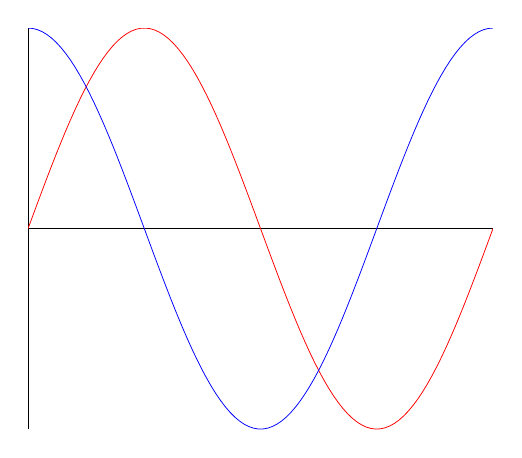
\begin{tikzpicture}[scale=0.7]
      \begin{axis}[
          scale only axis,
          no markers,
          domain=0:2*pi,
          samples=100,
          axis lines=center,
          axis line style={-},
          ticks=none]
        \addplot[red] {sin(deg(x))};
        \addplot[blue] {cos(deg(x))};
      \end{axis}
    \end{tikzpicture}
    \caption{The figure's caption}
  \end{figure}


\end{frame}


\begin{frame}{Full-slide sub-figure}

  \begin{figure}
  \begin{subfigure}[h]{0.45\textwidth}
    \centering
    \includegraphics[width=3cm]{assets/img/new_york_vanilla_info.png}
  \end{subfigure}
  \begin{subfigure}[h]{0.45\textwidth}
    \centering
    \includegraphics[width=3cm]{assets/img/new_york_simplified_roads.png}
  \end{subfigure}

   
  \end{figure}


\end{frame}